\chapter{Conception et implémentation de l’application}

\section{Conception}

\subsection{Introduction}
Tout comme la construction d’une maison nécessite des plans à différents niveaux (vision extérieure, plan des différents étages, plans techniques…), la réalisation d’une application informatique ou d’un ensemble d’applications est basée sur plusieurs diagrammes. Ces diagrammes doivent unifier la vision de l’équipe de développement et l’orienter vers la création d’une solution bien alignée sur les exigences du problème, et permettre également à l’équipe de proposer à ses clients une expérience utilisateur cohérente tout au long de l’application. 

Pour atteindre l'objectif de communiquer une vision ou un système difficile à expliquer par des mots, différents langages de modélisation ont été créés, tels que SysML, BON et le langage \acrshort{UML} le plus connu et le plus utilisé, ainsi que des méthodes anciennes et récentes, telles que le wireframing.

La pratique des conceptions logicielles n’est pas une pratique rigide dans laquelle plusieurs étapes clés sont toujours présentes dans un ordre particulier, par exemple : Le langage UML ne préconise aucune démarche, ce n’est donc pas une méthode. Chacun est libre d’utiliser les types de diagramme qu’il souhaite, dans l’ordre qu’il veut. Il suffit que les diagrammes réalisés soient cohérents entre eux, avant de passer à la réalisation du logiciel.

\subsection{Diagrammes de base}
\subsubsection{Diagrammes de séquence}

\begin{figure}[H]
	\centering
		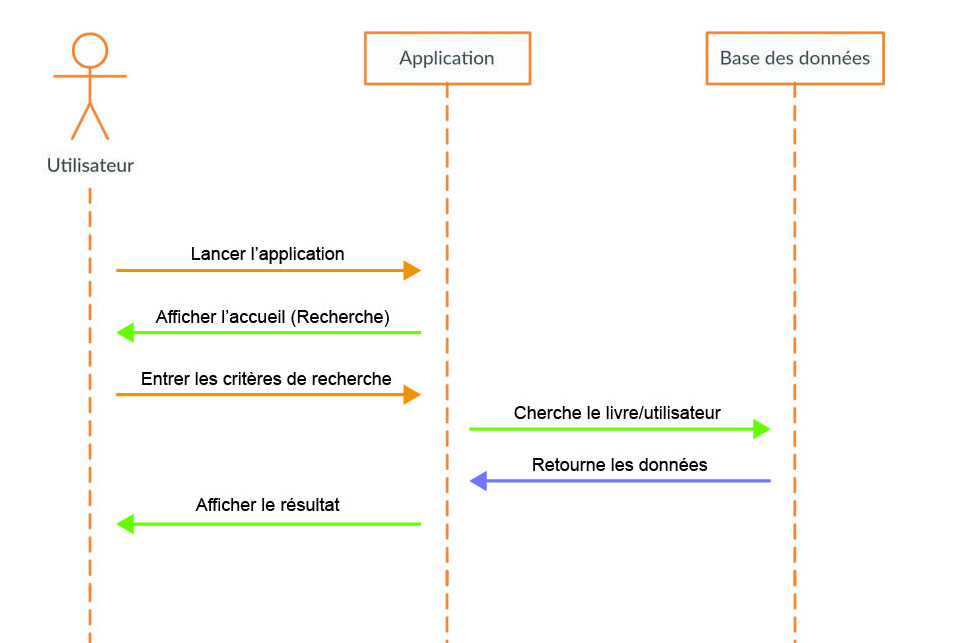
\includegraphics[width=10cm]{Images/chapter3/rechercher_un_livre.jpg}
		\caption{{\footnotesize l'enchaînement des actions pour la recherche d'un  livre particulier}}
\end{figure}

\begin{figure}[H]
	\centering
		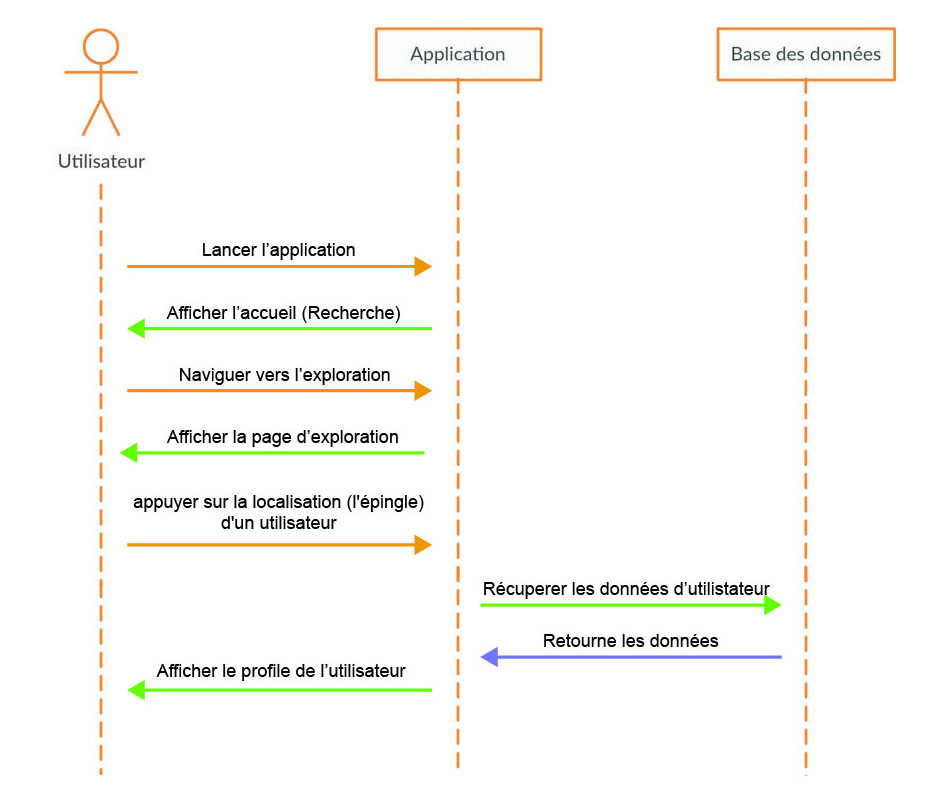
\includegraphics[width=10cm]{Images/chapter3/explorer_les_livres.jpg}
		\caption{{\footnotesize l'enchaînement des actions l'exploration des livres/utilisateurs à proximité}}
\end{figure}

\newpage

\subsubsection{Diagramme de navigation}

\begin{figure}[h]
	\begin{center}
		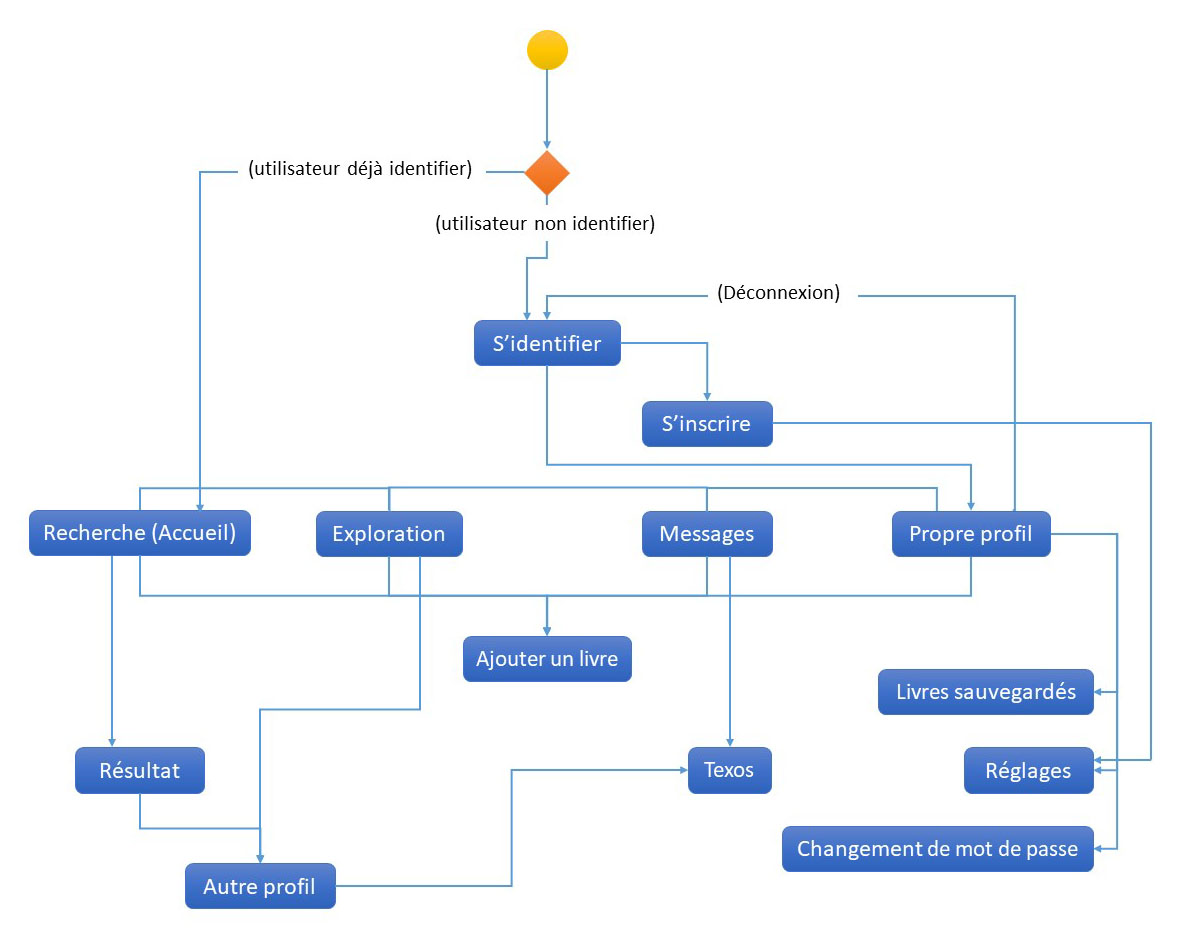
\includegraphics[width=14cm]{Images/chapter3/diagramme_de_navigation.jpg}
		\caption{{\footnotesize l'architecture de navigation}}
	\end{center}
\end{figure}

\newpage
\subsection{Maquette fonctionnelle (Wireframe)}
\subsubsection{Définition}
Le wireframe ou maquette fonctionnelle est un schéma utilisé lors de la conception d'une interface pour définir les zones et composants qu'elle doit contenir. À partir d'un wireframe peut être réalisée l'interface proprement dite par un graphiste. La démarche de recourir à des wireframes s'inscrit dans une recherche d'ergonomie. Elle est surtout utilisée dans le cadre du développement logiciel et des sites et applications Web. Le wireframe consiste concrètement en un croquis, un collage papier ou un schéma numérique\cite{noauthor_wireframe_nodate}.

\subsubsection{Les différentes écrans}
\begin{figure}[H]
	\begin{center}
		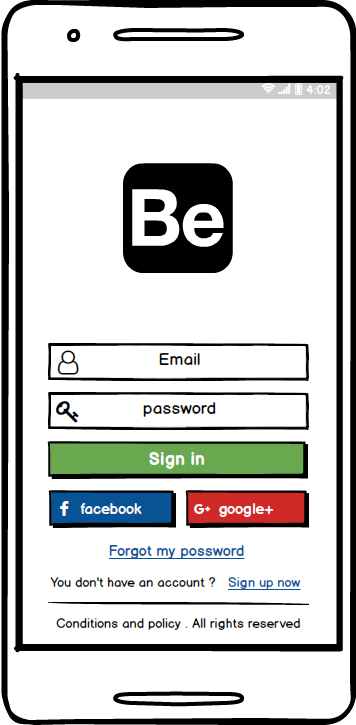
\includegraphics[height=8cm]{Images/chapter3/wireframe/sign_in.png}
		\caption{{\footnotesize Écran d'identification}}
	\end{center}
\end{figure}

\begin{figure}[H]
	\begin{center}
		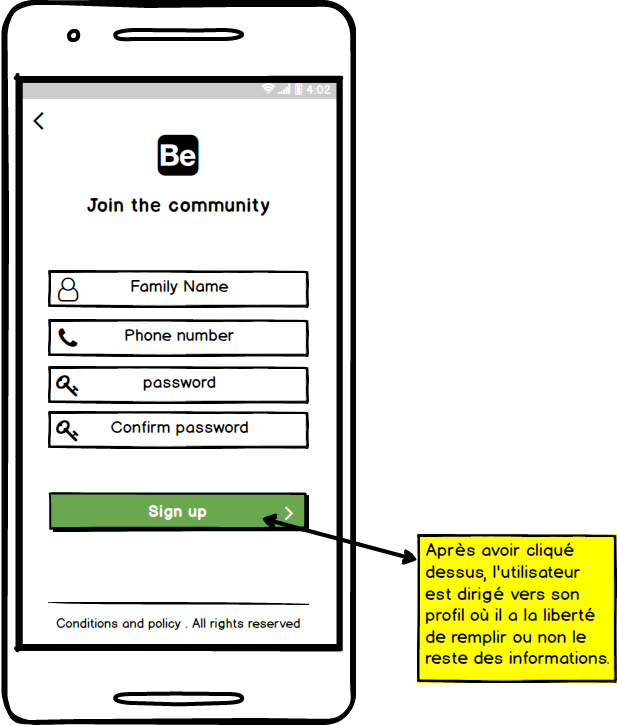
\includegraphics[height=8cm]{Images/chapter3/wireframe/sign_up.png}
		\caption{{\footnotesize Écran d'inscription}}
	\end{center}
\end{figure}

\begin{figure}[H]
	\begin{center}
		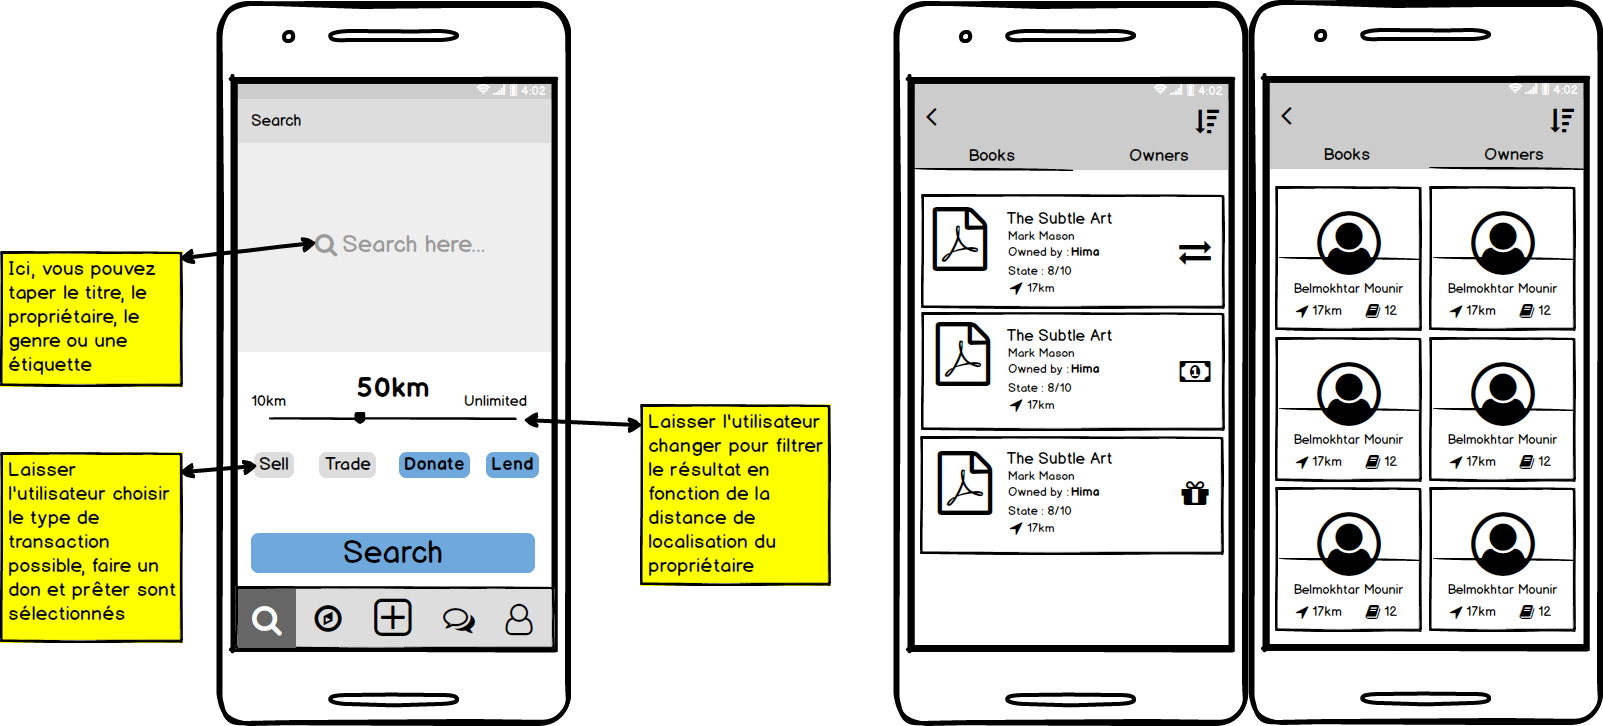
\includegraphics[width=14cm]{Images/chapter3/wireframe/home.png}
		\caption{{\footnotesize Écran de recherche (Accueil) + résultat}}
	\end{center}
\end{figure}

\begin{figure}[H]
	\begin{center}
		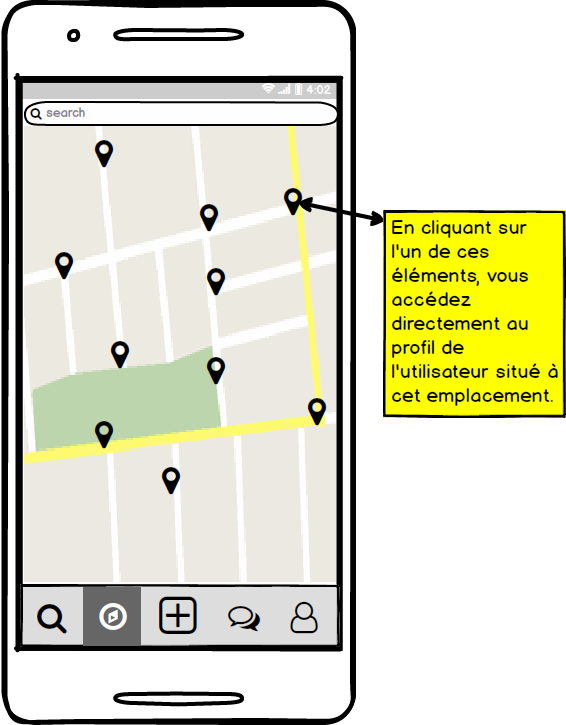
\includegraphics[height=8cm]{Images/chapter3/wireframe/explore.png}
		\caption{{\footnotesize Écran d'exploration}}
	\end{center}
\end{figure}

\begin{figure}[H]
	\begin{center}
		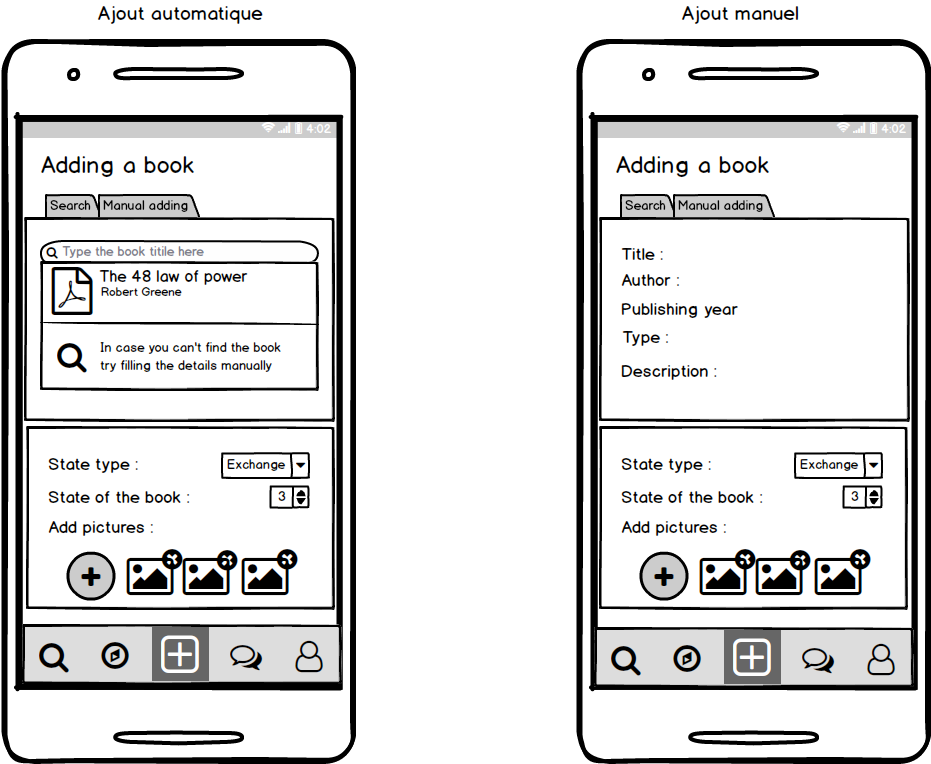
\includegraphics[height=8cm]{Images/chapter3/wireframe/adding_a_book.png}
		\caption{{\footnotesize Écran d'ajout des livres}}
	\end{center}
\end{figure}

\begin{figure}[H]
	\begin{center}
		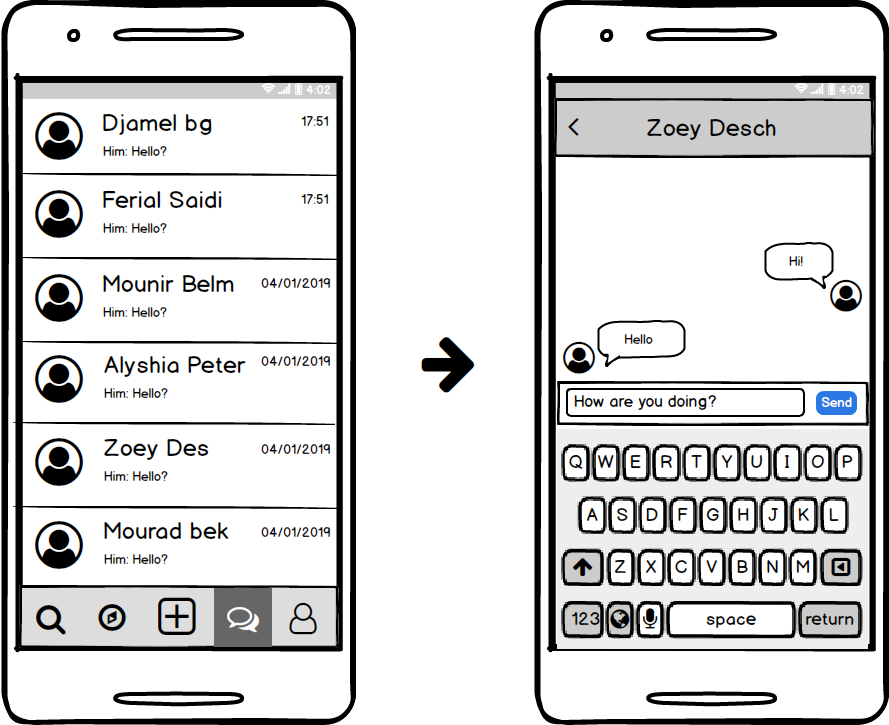
\includegraphics[height=8cm]{Images/chapter3/wireframe/messages.png}
		\caption{{\footnotesize Écran des messages + Textos}}
	\end{center}
\end{figure}

\begin{figure}[H]
	\begin{center}
		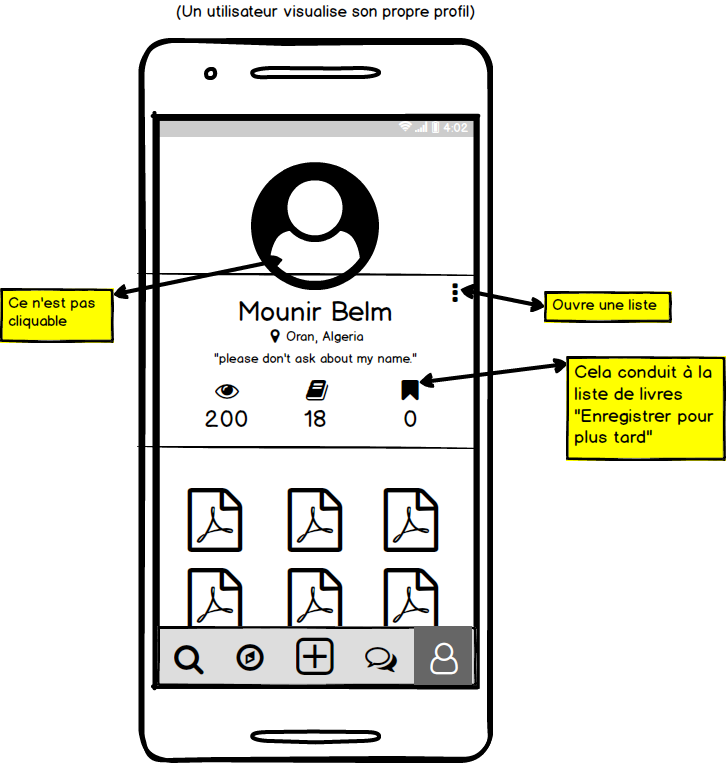
\includegraphics[height=8cm]{Images/chapter3/wireframe/profile.png}
		\caption{{\footnotesize Écran de profil de l'utilisateur authentifié}}
	\end{center}
\end{figure}

\begin{figure}[H]
	\begin{center}
		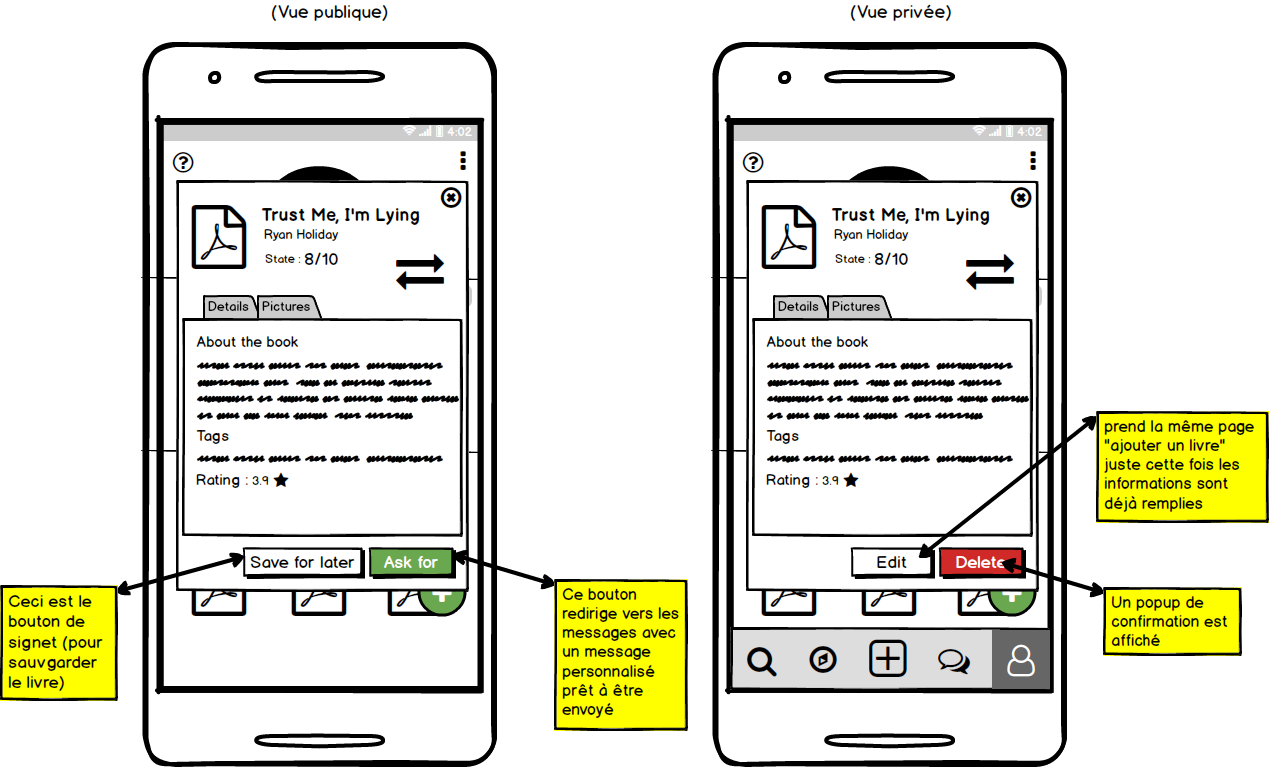
\includegraphics[height=8cm]{Images/chapter3/wireframe/displaying_a_book_details.png}
		\caption{{\footnotesize Fenêtre des détails de livre}}
	\end{center}
\end{figure}

\begin{figure}[H]
	\centering
		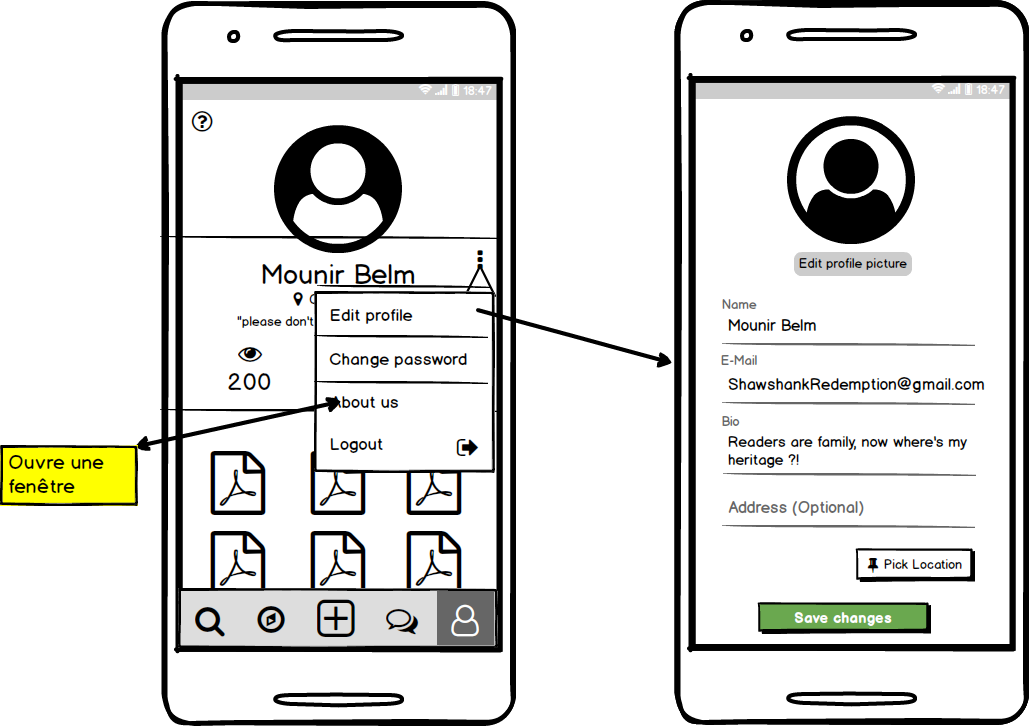
\includegraphics[height=8cm]{Images/chapter3/wireframe/settings.png}
		\caption{{\footnotesize Écran des réglages}}
\end{figure}

\begin{figure}[H]
	\centering
		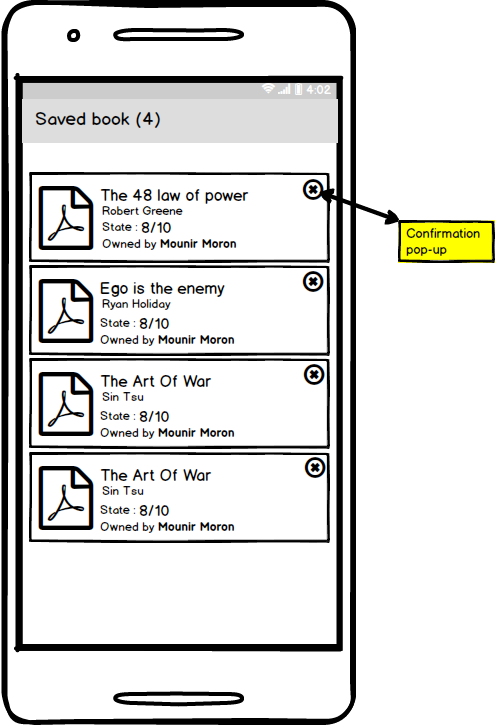
\includegraphics[height=8cm]{Images/chapter3/wireframe/saved_for_later.png}
		\caption{{\footnotesize Écran des livres sauvegardes}}
\end{figure}

\begin{figure}[H]
	\centering
		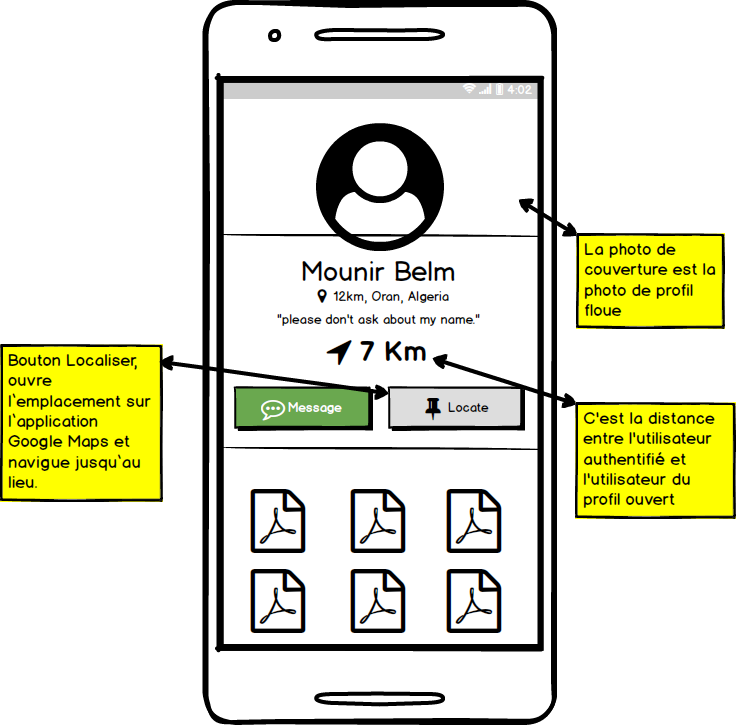
\includegraphics[height=8cm]{Images/chapter3/wireframe/other_profile.png}
		\caption{{\footnotesize Écran de profil d'un autre utilisateur}}
\end{figure}

\newpage

\subsubsection{Outil utilisé (Balsamiq Mockups)}

\begin{wrapfigure}[5]{r}{2cm}
	
\includegraphics[width=2cm]{Images/chapter3/balsamiq_logo.png}
	\vspace{-20pt}
	\caption{{\footnotesize Logo de Balsamiq}}
\end{wrapfigure}

Balsamiq Mockups est un outil de conception d'interface utilisateur permettant de créer des structures filaires (également appelées maquettes ou prototypes basse fidélité). Vous pouvez l'utiliser pour générer des esquisses numériques de vos idées de produits afin de faciliter la discussion et la compréhension avant l'écriture de tout code.\cite{noauthor_balsamiq_nodate}\\\\

\begin{figure}[h]
	\centering
		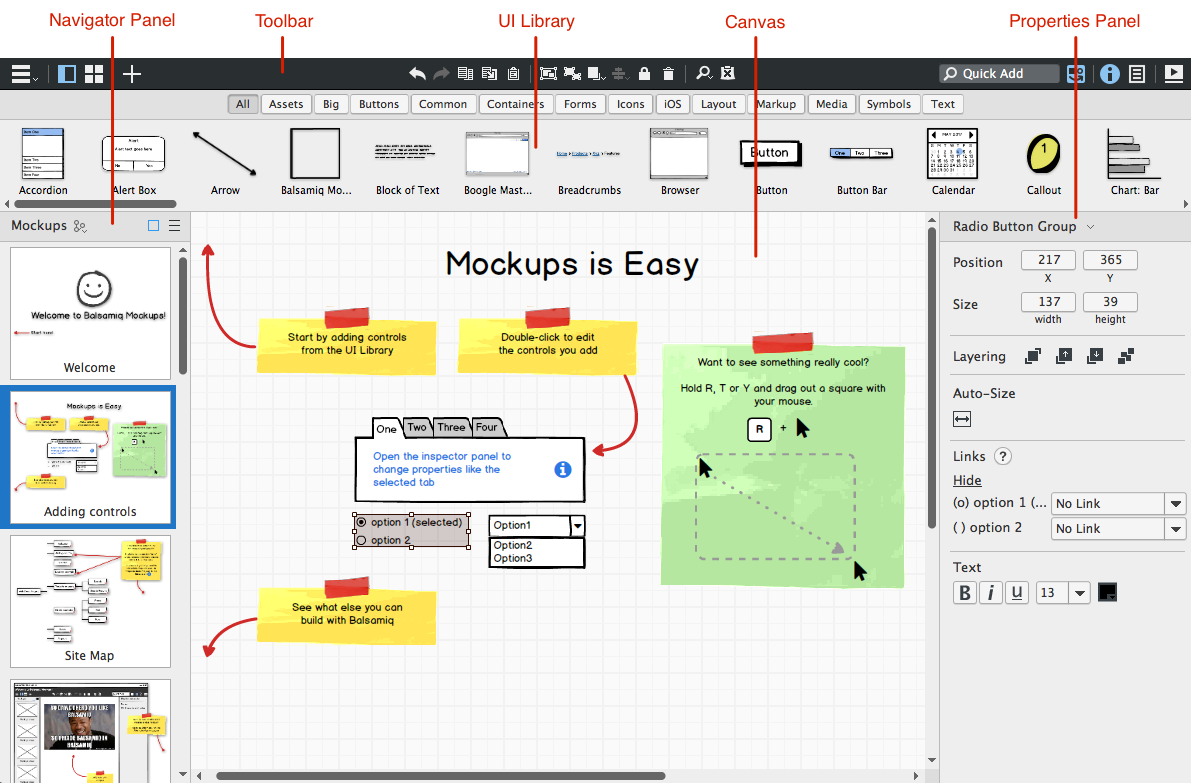
\includegraphics[width=14cm]{Images/chapter3/balsamiq_ui_overview.png}
		\caption{{\footnotesize l'interface de Balsamiq Mockups}}
\end{figure}


\newpage
\subsection{Prototypage logiciel}
\subsubsection{Introduction}
Les équipes de développement sont généralement peu disposées à mettre en œuvre une phase de prototypage pour concevoir l’interface, car elles craignent de devoir en attendre la fin pour démarrer effectivement le développement, rallongeant d’autant le planning du projet. Pourtant, il peut être judicieux d'intégrer le prototypage dans la phase de spécification fonctionnelle, afin de valider puis définir les exigences et comportements à développer. De même, il est possible de jouer sur la fidélité du prototype, c’est-à-dire sa ressemblance par rapport au produit final en termes d’interactivité et de graphisme.

Et pour cela, nous avons décidé de créer un prototype afin de tester l'interactivité de la solution et de chercher plus en détail les défauts qui n'auraient peut-être pas été découverts au cours des phases initiales du conception. En outre, le projet étant un travail combiné de deux étudiants, nous avions besoin d’un chemin clair et précis à suivre pendant la phase de développement.

Nous avons utilisé le type de prototypage horizontal, tout en respectant les directives de Material Design. Pour l'outil, la solution la plus appropriée était Adobe XD. Toutes ces solutions seront décrites plus en détail dans les sections suivantes.

\subsubsection{Définition}
Le prototypage logiciel est l’activité de création de prototypes d’applications logicielles, c’est-à-dire des versions incomplètes du programme logiciel en cours de développement. C’est une activité qui peut exister dans le développement de logiciels et qui est comparable au prototypage connu dans d’autres domaines, tels que le génie mécanique ou la fabrication.

Un prototype ne simule généralement que quelques aspects du produit final et peut être complètement différent de celui-ci\cite{noauthor_software_nodate}.

\subsubsection{Le prototype horizontal}
Le prototypage consiste à concevoir des versions intermédiaires et donc incomplètes d'un logiciel ou d'un site web, conçues pour tester l'utilisation avant la phase proprement dite de programmation informatique. Dans le cadre d'une intervention ergonomique, la phase de prototypage permet de tester l'utilisation et l'utilisabilité d'un produit auprès d'utilisateurs (test utilisateur). Il se distingue de la maquette fil de fer (ou wireframe) en simulant le fonctionnement avec des données fictives ou réelles. Plusieurs types et niveaux de finition sont possibles, selon la démarche de conception d'un logiciel ou d'un site Web. Le prototypage s’inscrit dans une démarche de conception itérative de l’interface, en particulier dans la démarche de conception centrée sur l'utilisateur. Il vise à améliorer progressivement l’interface en s’appuyant sur l’analyse du comportement des utilisateurs finaux lorsqu'ils se servent du produit\cite{noauthor_prototypage_nodate}.

\subsubsection{Material Design}

Le Material Design est un ensemble de règles de design proposées par Google et qui s'appliquent à l'interface graphique des logiciels et applications. Il est utilisé notamment à partir de la version 5.0 du système d'exploitation Android.

Google a présenté le Material Design pour la première fois lors de la conférence Google I/O, le 25 juin 2014. En misant sur les motifs « carte », déjà utilisés dans Google Now, ces règles de design mettent l'accent sur une utilisation accrue des mises en page basées sur une grille, des animations et des transitions, des effets de profondeur tels l'éclairage et les ombres. Selon Google ce nouveau langage de design est basé sur le papier et l'encre.

Le designer Matías Duarte explique que « contrairement au vrai papier, notre matériau numérique peut s'étirer et se modifier de manière intelligente. Le matériau contextuel a une surface physique et des bords. Les superpositions et les ombres donnent des informations sur ce que vous pouvez toucher ».\cite{noauthor_material_2018}.

\begin{figure}[H]
	\centering
		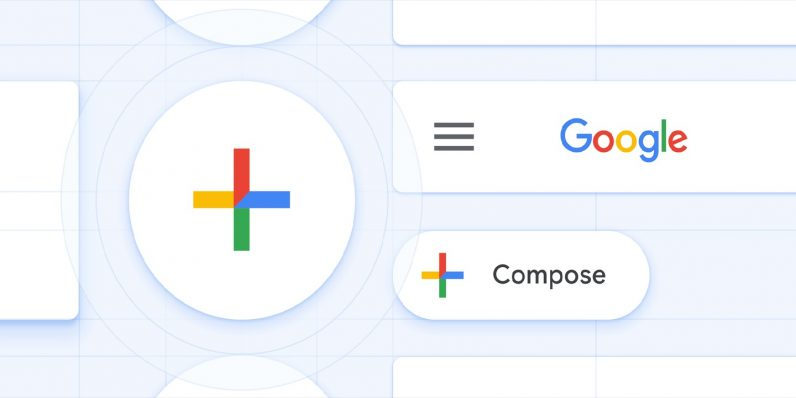
\includegraphics[width=14cm]{Images/chapter3/material_design.jpg}
		\caption{{\footnotesize Des composents d'interface graphique respectants les règles de Material Design}}
\end{figure}

\subsubsection{Outil utilisé (Adobe Xd)}

\begin{wrapfigure}[10]{r}{3cm}
	\vspace{-10pt}
	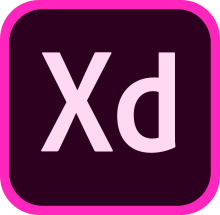
\includegraphics[width=3cm]{Images/chapter3/adobe_xd_logo.png}
	\vspace{-10pt}
	\caption{{\footnotesize Logo de Adobe Xd}}
\end{wrapfigure}

Adobe XD est un outil vectoriel développé et publié par Adobe Inc pour la conception et la prototypage de l'expérience utilisateur pour les applications Web et mobiles. Le logiciel est disponible pour macOS, Windows, iOS et Android.

Adobe a annoncé pour la première fois qu'il développait un nouvel outil de conception et de prototypage d'interface sous le nom de "Project Comet" lors de la conférence Adobe MAX en octobre 2015. La première version bêta publique a été publiée pour macOS en tant que "Adobe Experience Design CC" pour les utilisateurs disposant d'un compte Adobe le 14 mars 2016. Une version bêta d'Adobe XD est sortie pour Windows 10 le 13 décembre 2016. Le 18 octobre 2017, Adobe a annoncé qu'Adobe XD n'était plus en version bêta.

Cet outil permet aux utilisateurs de créer des interfaces utilisateur pour les applications mobiles et Web. XD offre de nombreuses fonctionnalités permettant un design et des fonctionnalités créatifs. Auparavant, de nombreuses fonctionnalités de XD étaient difficiles à utiliser ou inexistantes dans d’autres applications de conception Adobe telles que Illustrator ou Photoshop. Adobe XD est livré avec des kits d'interface utilisateur pour Apple iOS, Microsoft Windows et Google Material Design déjà intégrés.\cite{noauthor_adobe_2019}

\begin{figure}[H]
	\centering
		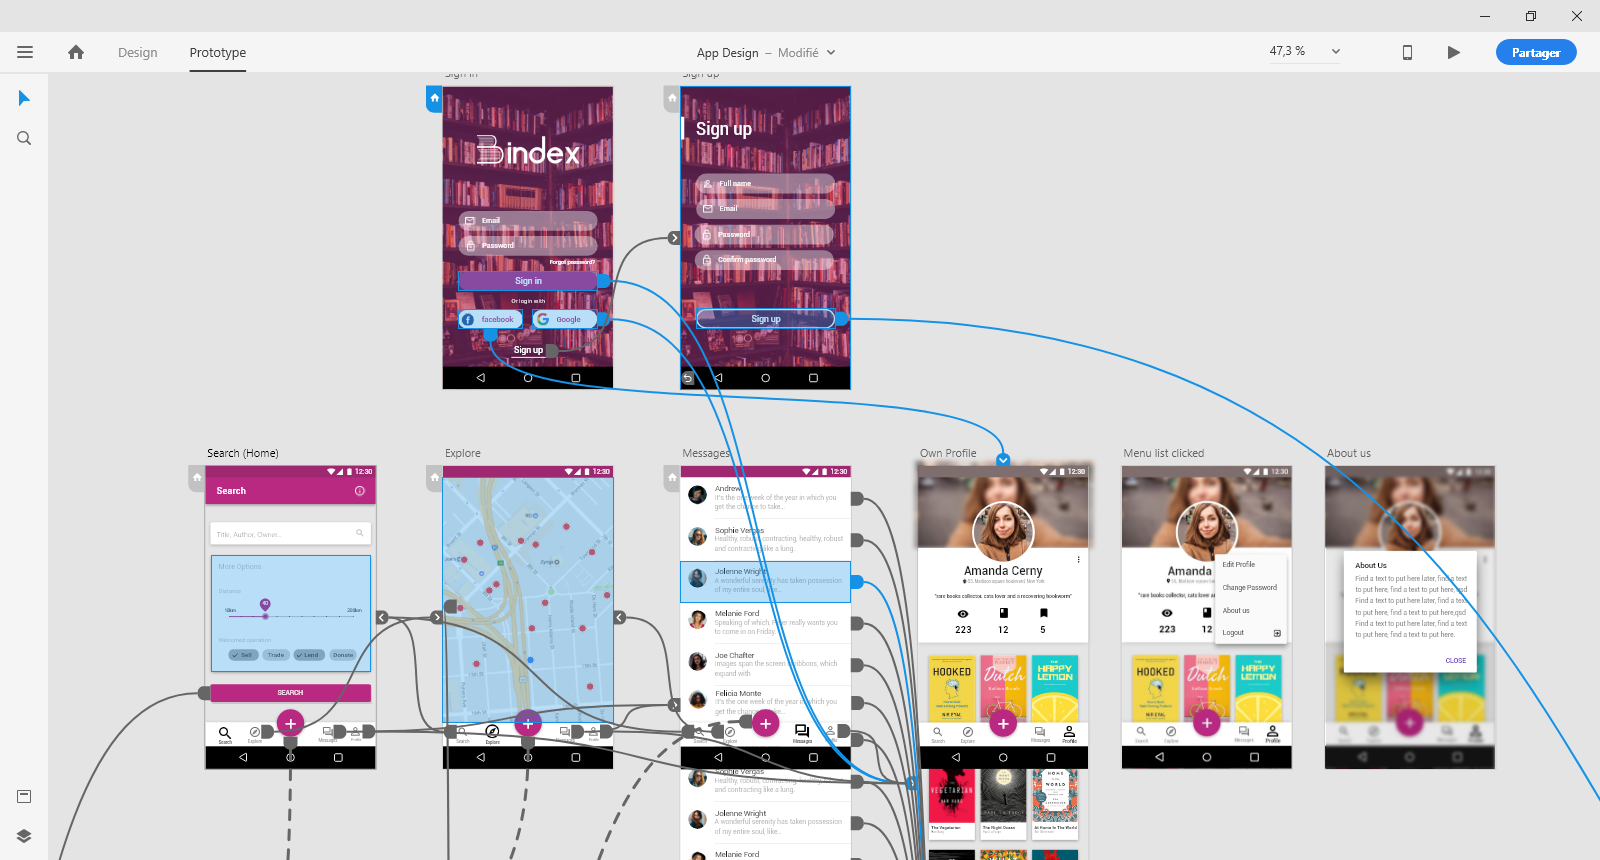
\includegraphics[width=14cm]{Images/chapter3/adobe_xd_interface.png}
		\caption{{\footnotesize l'interface de Adobe Xd}}
\end{figure}

\subsubsection{La maquette de prototype (UI Design)}

\begin{figure}[H]
	\centering
		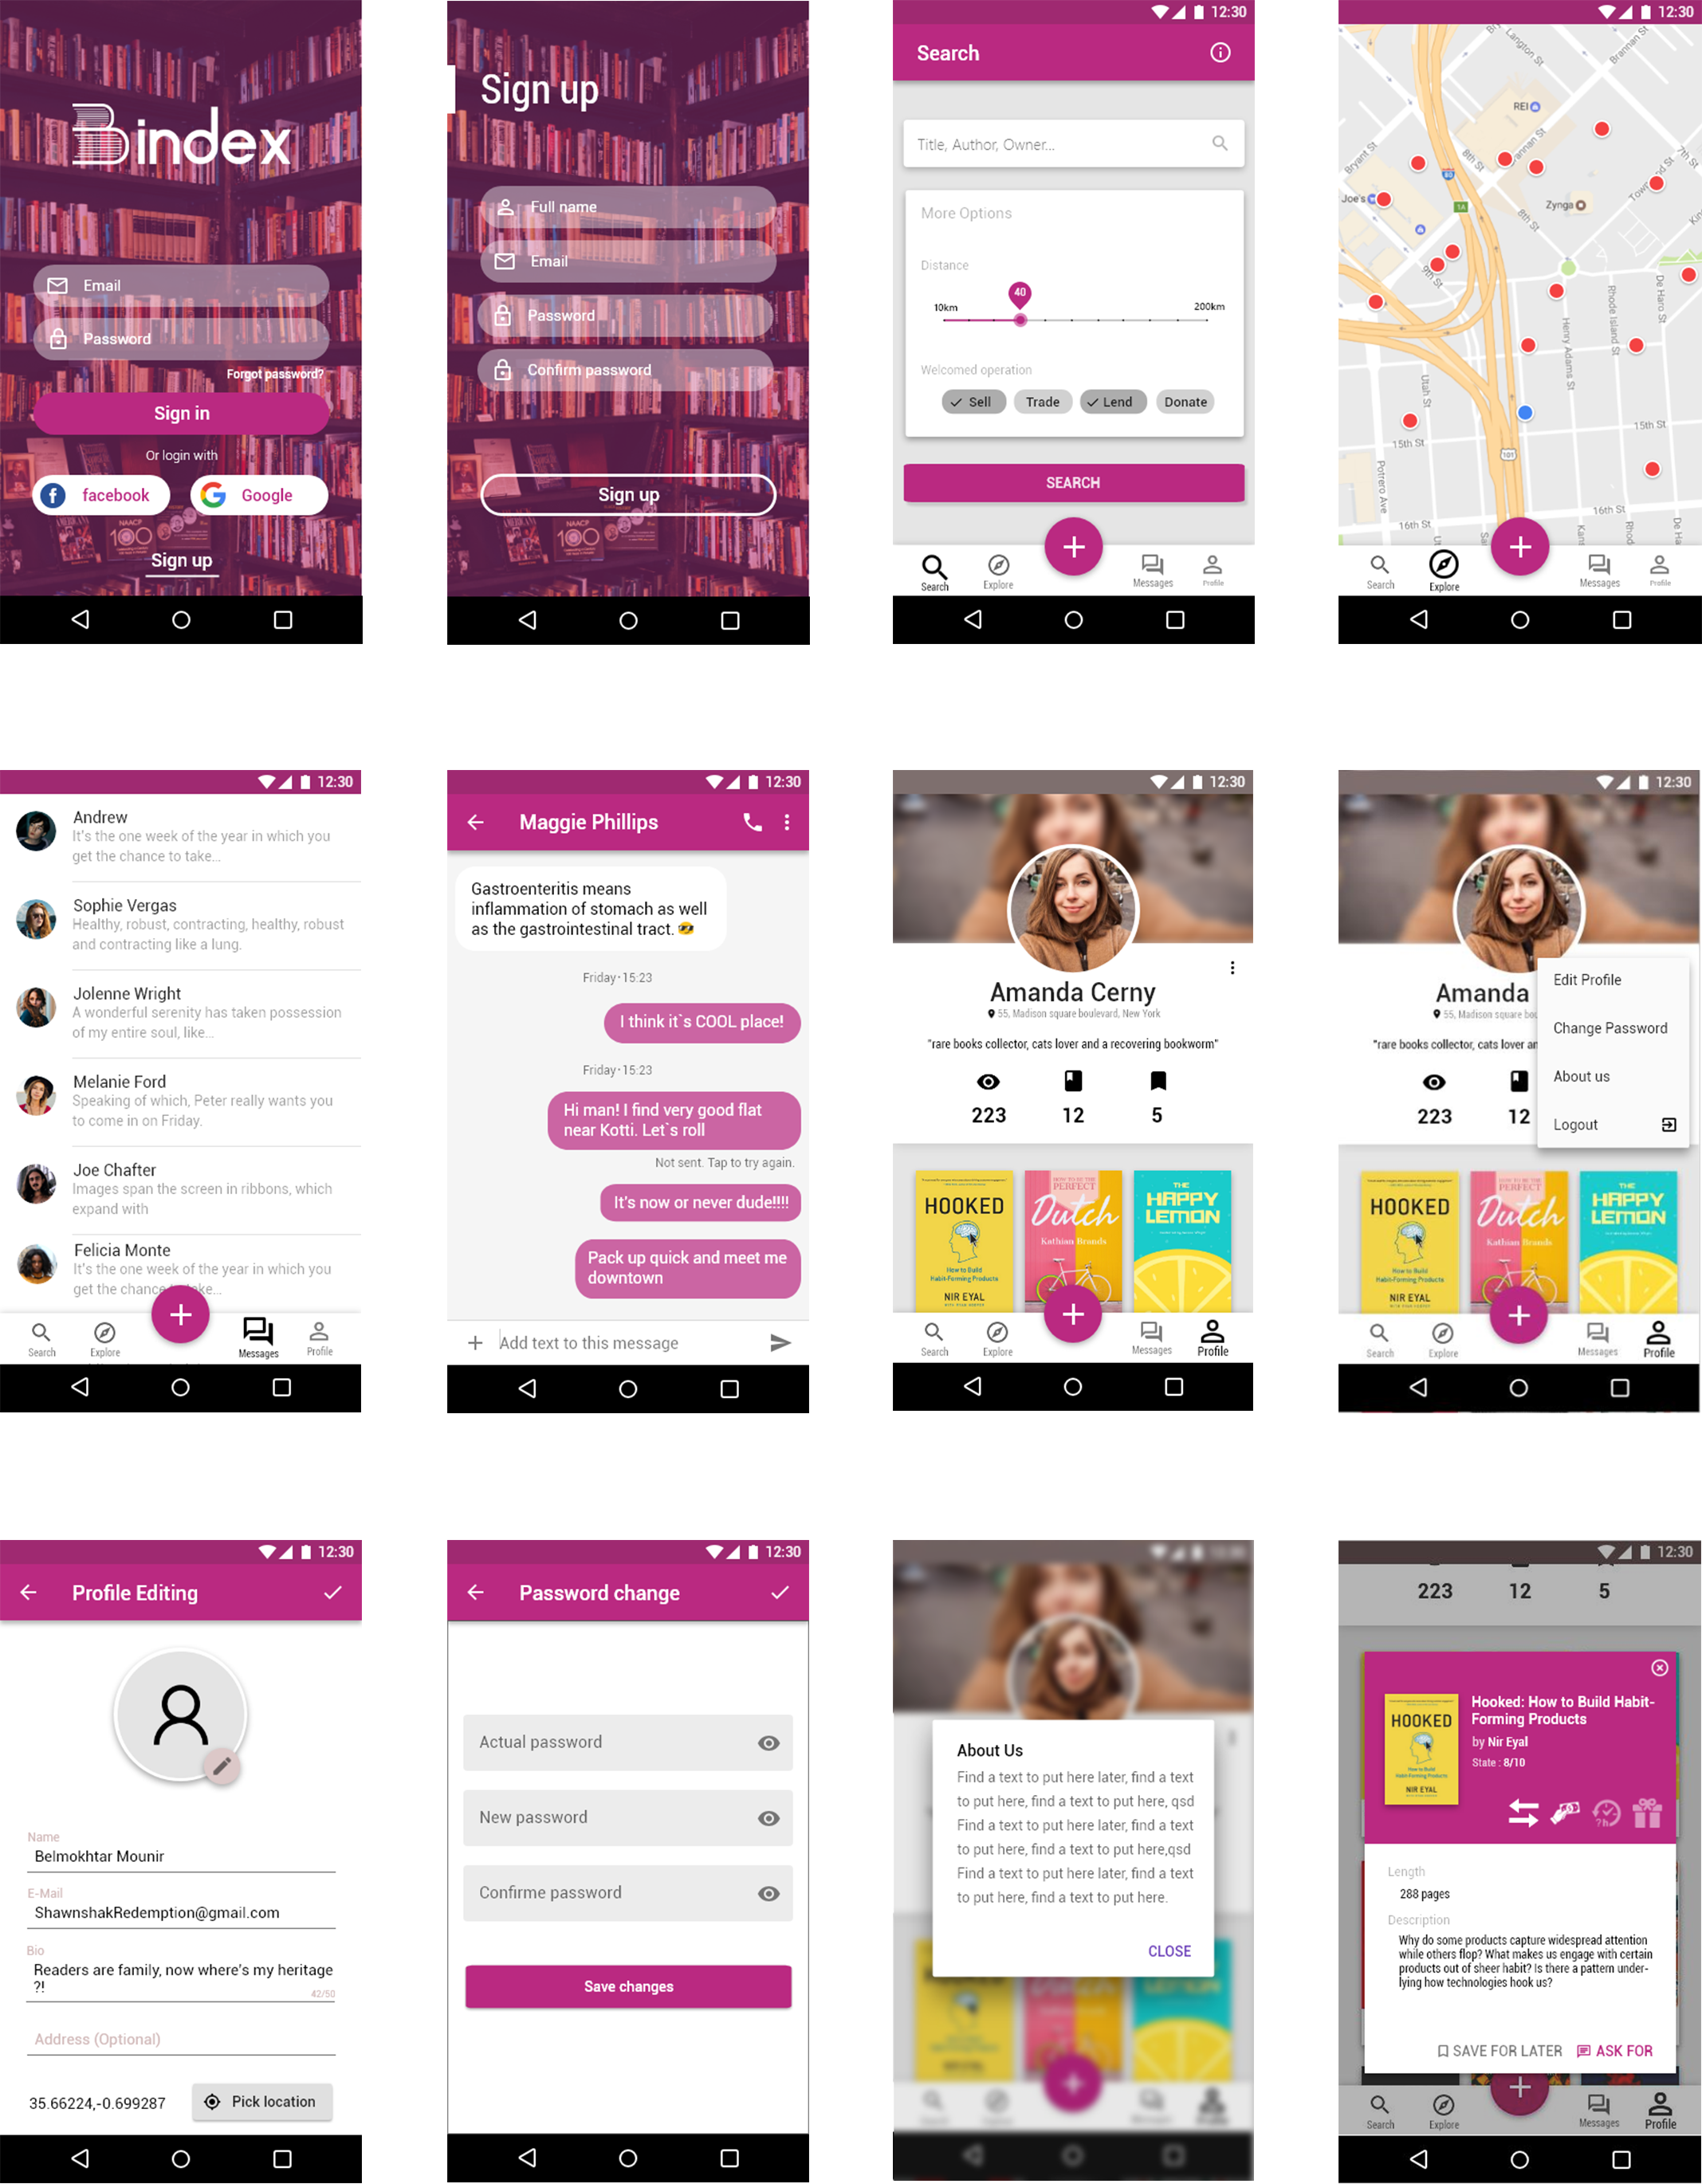
\includegraphics[width=14cm]{Images/chapter3/ui-design_1.png}
\end{figure}

\begin{figure}[H]
	\centering
		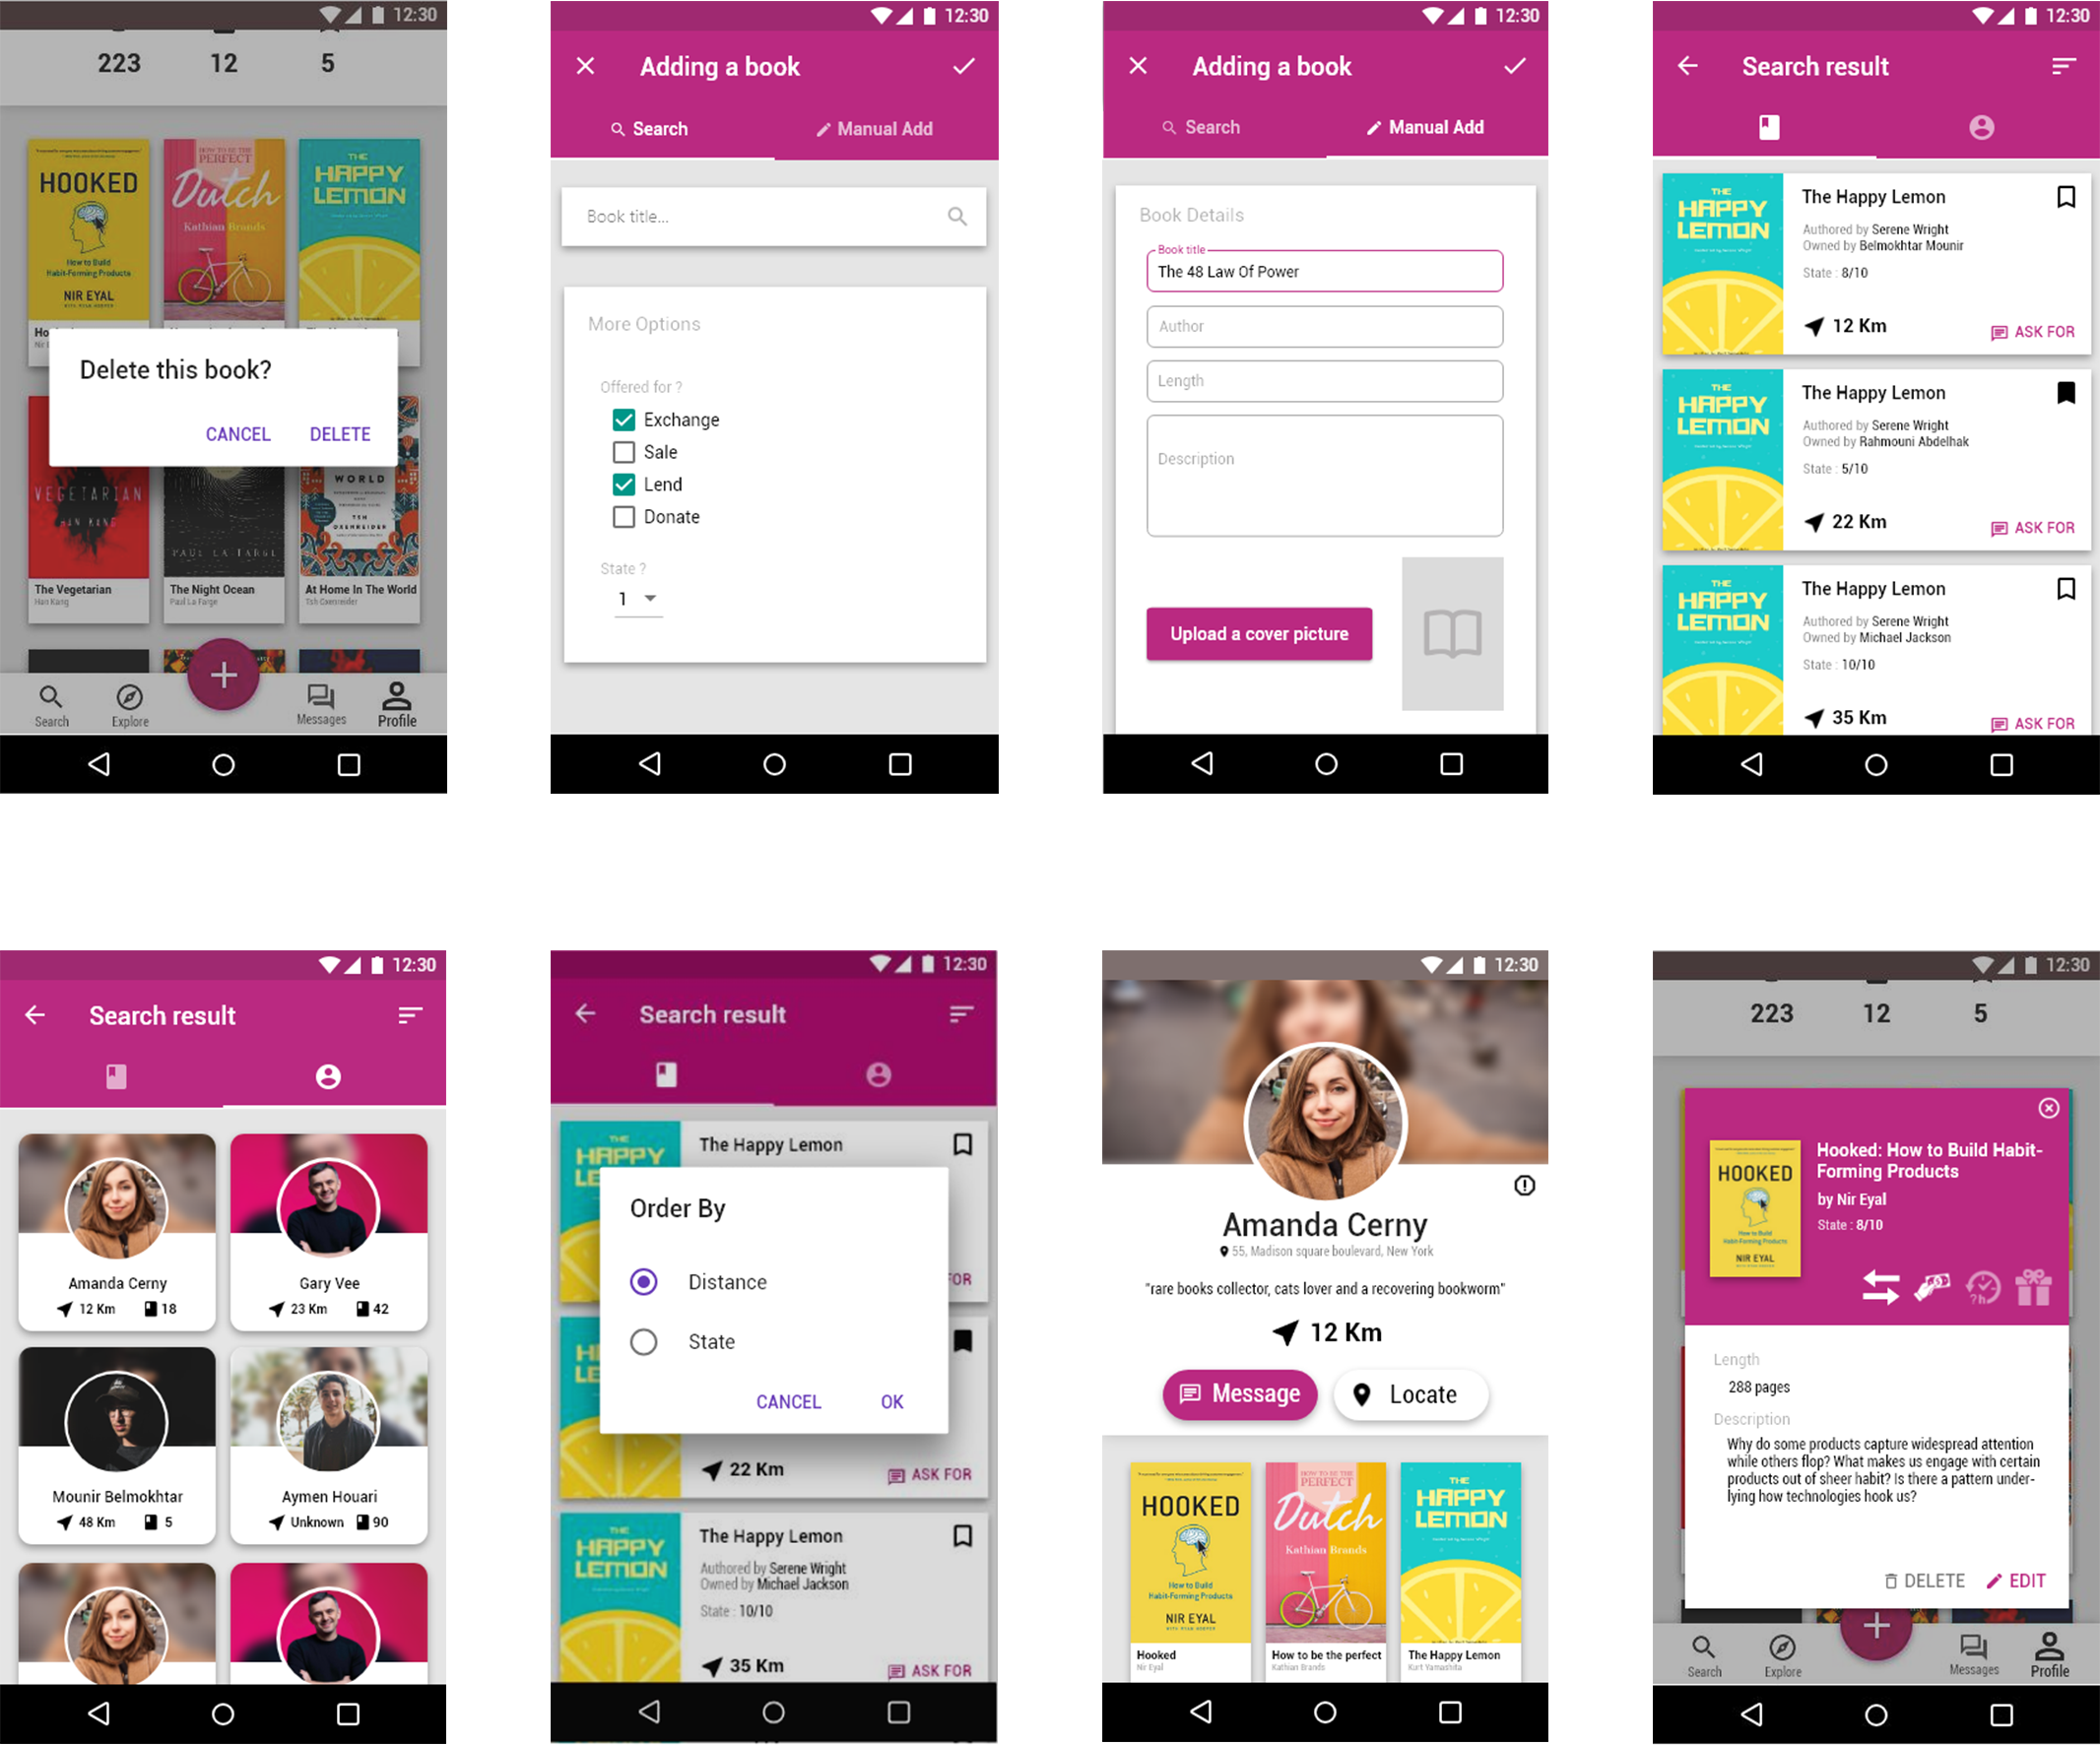
\includegraphics[width=14cm]{Images/chapter3/ui-design_2.png}
		\caption{{\footnotesize Le design des différentes écrans de l'application}}
\end{figure}

\newpage

\section{Implémentation}
\subsection{Introduction}
Après la phase de conception, vient la mise en œuvre, qui consiste en une série d’actions aboutissant à un logiciel entièrement formé à la fin, tout en respectant les restrictions et les descriptions convenues lors de la phase précédente.

\subsection{Structure de l'application}

\begin{figure}[H]
	\centering
		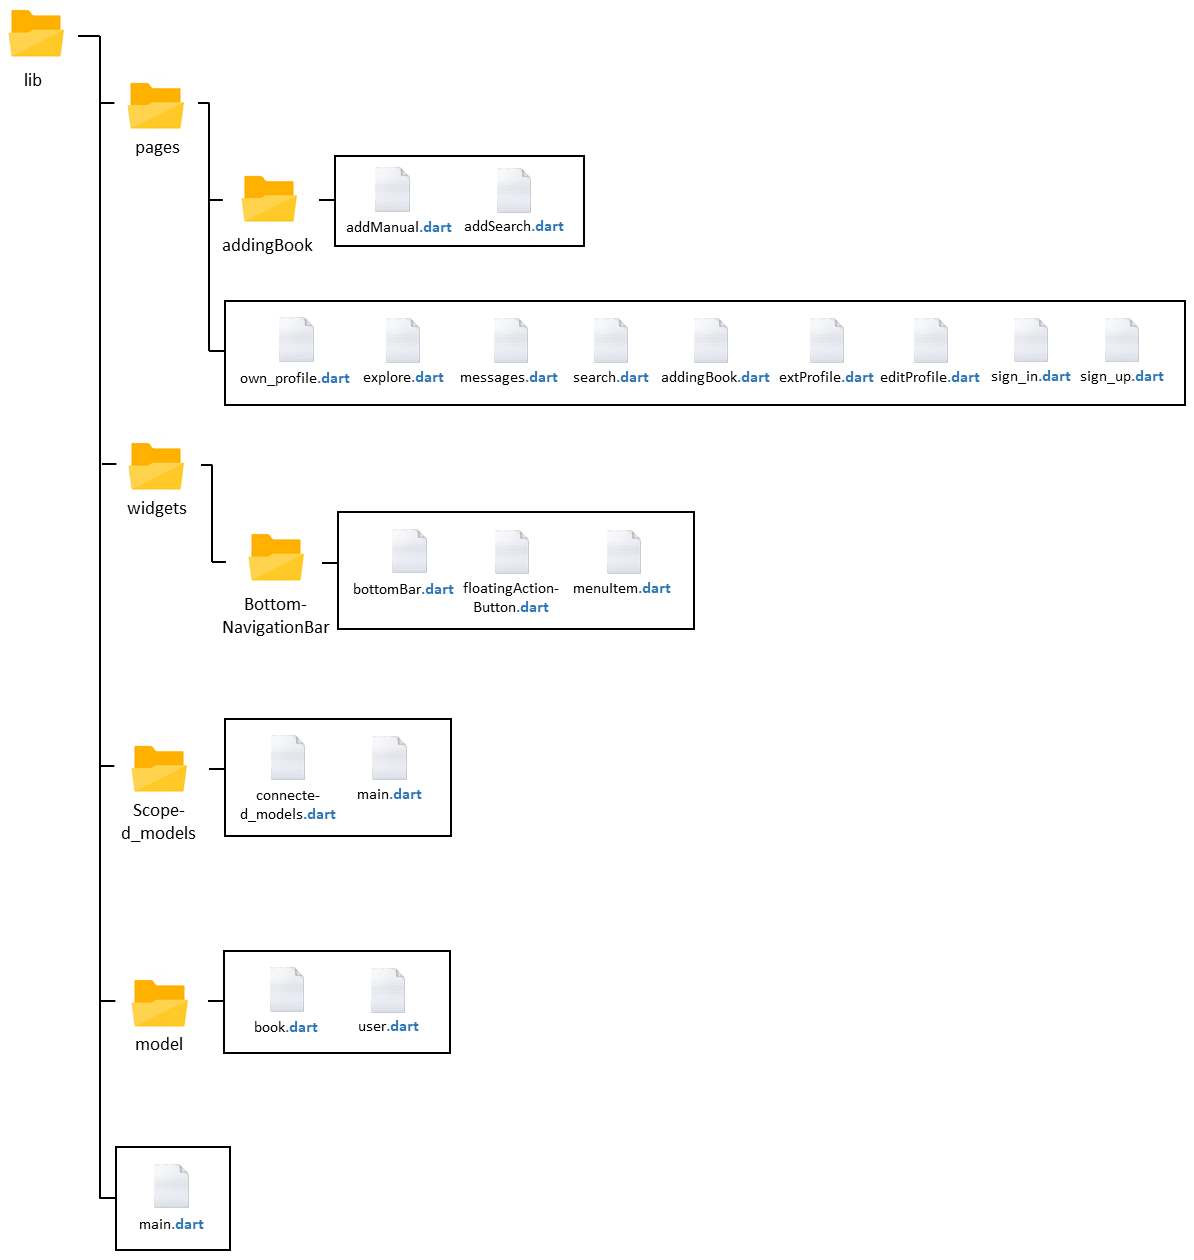
\includegraphics[width=13cm]{Images/chapter3/software_architecture.png}
		\caption{{\footnotesize La structure des fichiers sources}}
\end{figure}

\newpage

\subsubsection{Architecture de gestion des états}
Dans le but de créer une application facile à gérer, nous avons choisi l’architecture Scoped Model qui est basé sur un package tiers qui n'est pas inclus dans le framework Flutter. Voici comment les développeurs de Scoped Model le décrivent:

\begin{quote}
Un ensemble d’utilitaires vous permettant de facilement passer un modèle de données d’un Widget parent à ses descendants. En outre, il reconstruit également tous les enfants qui utilisent le modèle lors de la mise à jour du modèle. Cette bibliothèque a été extraite de la base de code Fuchsia
\end{quote}

Avec scoped\_model, il est beaucoup plus facile de travailler avec l’état dans votre application.
Même si l'utilisation exclusive de StatefulWidget est une excellente chose, la plupart du temps, votre application aura plusieurs widgets qui doivent utiliser le même état partagé. Le problème, c’est que lorsque ces widgets existent à différents endroits de notre application, la transmission de l’état devient assez fastidieuse.

En d'autres termes, scoped\_model permet à différents widgets d'accéder facilement au même état partagé.

Il y a aussi quelques avantages supplémentaires intéressants que vous obtenez:

\begin{list}{•}{}
\item Cela nous permet de consolider facilement les variables d'état et la logique métier de l'ensemble de l'application.
\item Nous pouvons éviter de lire sur des modèles d'architecture trop complexes.
\item Un code passe-partout minimal est requis par rapport à des bibliothèques similaires.
\end{list}

\newpage

\subsection{Les outils utilisé}

\subsubsection{Android Studio}

\begin{wrapfigure}[11]{r}{3cm}
	\vspace{-10pt}
	
\includegraphics[width=3cm]{Images/chapter3/android_studio_icon.png}
	\vspace{-10pt}
	\caption{{\footnotesize Logo de Android Studio}}
\end{wrapfigure}

Android Studio est l'environnement officiel de développement intégré (\acrshort{IDE}) du système d'exploitation Android de Google, construit sur le logiciel IntelliJ IDEA de JetBrains et spécialement conçu pour le développement Android. Il est disponible au téléchargement sur les systèmes d'exploitation Windows, macOS et Linux. Il remplace les outils de développement Eclipse Android (ADT) comme IDE principal pour le développement d'applications Android natives.

Android Studio a été annoncé le 16 mai 2013 lors de la conférence Google I / O. C'était au début de la phase de prévisualisation de l'accès à partir de la version 0.1 en mai 2013, puis en phase bêta à partir de la version 0.8 publiée en juin 2014. La première version stable a été publiée en décembre 2014 à partir de la version 1.0.

Depuis le 7 mai 2019, Kotlin est la langue préférée de Google pour le développement d'applications Android. Néanmoins, d’autres langues sont prises en charge, notamment par Android Studio \cite{noauthor_android_nodate}.

\begin{figure}[H]
	\centering
		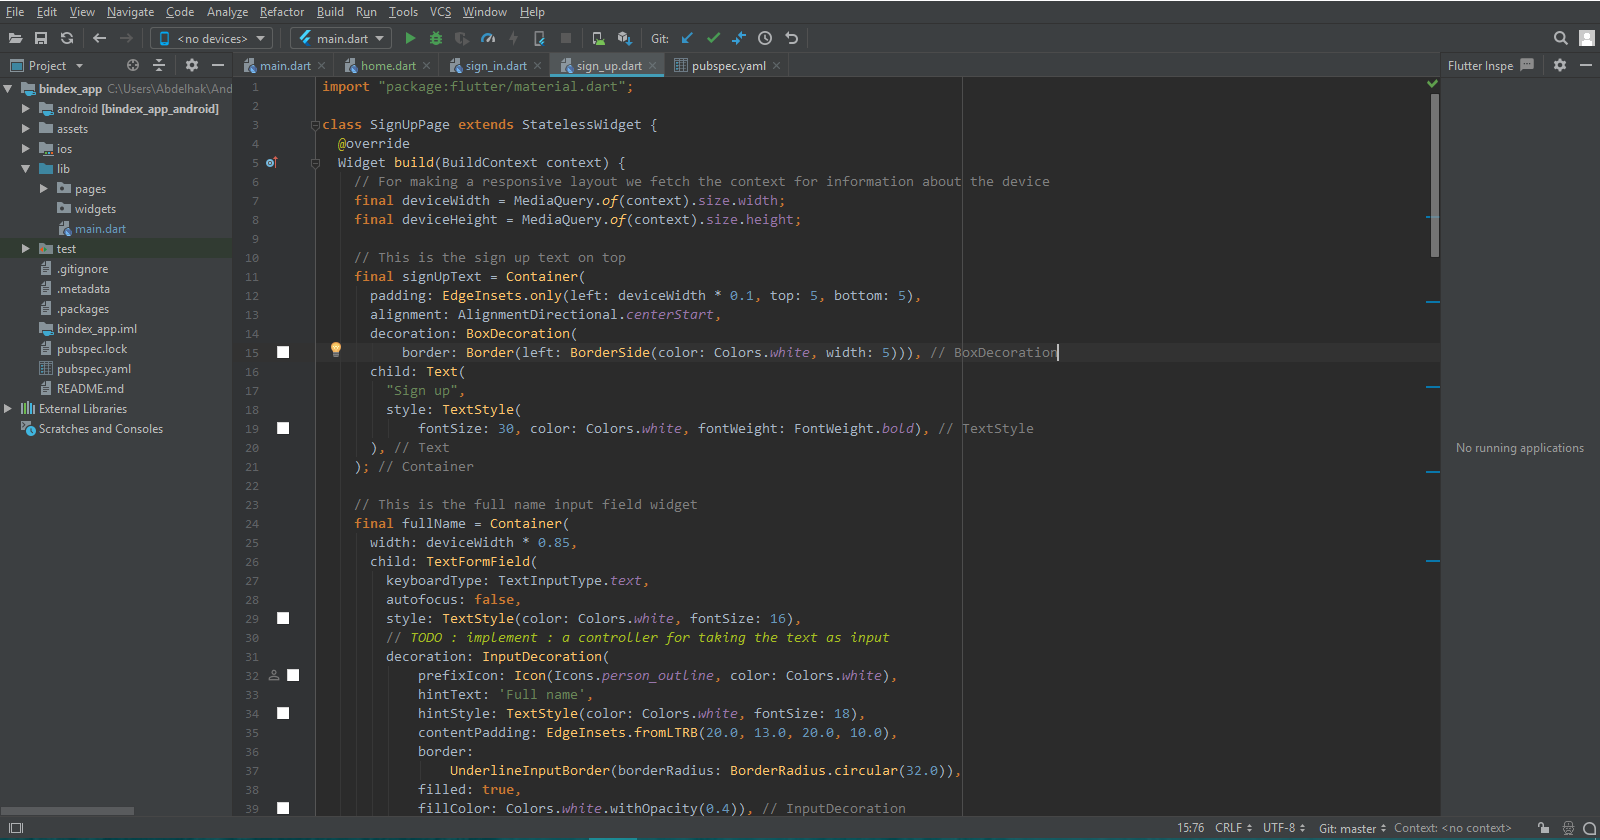
\includegraphics[width=14cm]{Images/chapter3/android_studio_interface.png}
		\caption{{\footnotesize l'interface de Android Studio}}
\end{figure}

\newpage

\subsubsection{Git}

\begin{wrapfigure}[7]{r}{3cm}
	
\includegraphics[width=3cm]{Images/chapter3/git_logo.png}
	\vspace{-10pt}
	\caption{{\footnotesize Logo de git}}
\end{wrapfigure}

Git est un système de contrôle de version distribué permettant de suivre les modifications du code source au cours du développement du logiciel. 
Il est conçu pour coordonner le travail des programmeurs, mais il peut être utilisé pour suivre les modifications dans n’importe quel ensemble de fichiers. Ses objectifs incluent la rapidité, l'intégrité des données et la prise en charge des flux de travail distribués non linéaires.

Git a été créé par Linus Torvalds en 2005 pour développer le noyau Linux. D'autres développeurs du noyau ont contribué à son développement initial. Son responsable actuel depuis 2005 est Junio Hamano.

Comme avec la plupart des systèmes de contrôle de version distribués, et contrairement à la plupart des systèmes client-serveur, chaque répertoire Git sur chaque ordinateur est un référentiel complet doté d'un historique complet et de capacités de suivi de version complètes, indépendant de l'accès réseau ou d'un serveur central.

Git est un logiciel gratuit et à code source ouvert distribué sous les termes de la licence publique générale GNU version 2 \cite{noauthor_git_nodate}